\documentclass[12pt,spanish,]{scrartcl}
\usepackage{lmodern}
\usepackage{amssymb,amsmath}
\usepackage{ifxetex,ifluatex}
\usepackage{fixltx2e} % provides \textsubscript
\ifnum 0\ifxetex 1\fi\ifluatex 1\fi=0 % if pdftex
  \usepackage[T1]{fontenc}
  \usepackage[utf8]{inputenc}
\else % if luatex or xelatex
  \ifxetex
    \usepackage{mathspec}
  \else
    \usepackage{fontspec}
  \fi
  \defaultfontfeatures{Ligatures=TeX,Scale=MatchLowercase}
    \setmainfont[]{Ubuntu}
    \setmonofont[Mapping=tex-ansi]{Ubuntu Mono}
\fi
% use upquote if available, for straight quotes in verbatim environments
\IfFileExists{upquote.sty}{\usepackage{upquote}}{}
% use microtype if available
\IfFileExists{microtype.sty}{%
\usepackage{microtype}
\UseMicrotypeSet[protrusion]{basicmath} % disable protrusion for tt fonts
}{}
\usepackage[a4paper]{geometry}
\usepackage[unicode=true]{hyperref}
\PassOptionsToPackage{usenames,dvipsnames}{color} % color is loaded by hyperref
\hypersetup{
            pdftitle={Probando la Orange Pi},
            pdfauthor={Sergio Alvariño sergio.alvarino@vodafone.com},
            colorlinks=true,
            linkcolor=Maroon,
            citecolor=Blue,
            urlcolor=Blue,
            breaklinks=true}
\urlstyle{same}  % don't use monospace font for urls
\ifnum 0\ifxetex 1\fi\ifluatex 1\fi=0 % if pdftex
  \usepackage[shorthands=off,main=spanish]{babel}
\else
  \usepackage{polyglossia}
  \setmainlanguage[]{spanish}
\fi
\usepackage{graphicx,grffile}
\makeatletter
\def\maxwidth{\ifdim\Gin@nat@width>\linewidth\linewidth\else\Gin@nat@width\fi}
\def\maxheight{\ifdim\Gin@nat@height>\textheight\textheight\else\Gin@nat@height\fi}
\makeatother
% Scale images if necessary, so that they will not overflow the page
% margins by default, and it is still possible to overwrite the defaults
% using explicit options in \includegraphics[width, height, ...]{}
\setkeys{Gin}{width=\maxwidth,height=\maxheight,keepaspectratio}
\IfFileExists{parskip.sty}{%
\usepackage{parskip}
}{% else
\setlength{\parindent}{0pt}
\setlength{\parskip}{6pt plus 2pt minus 1pt}
}
\setlength{\emergencystretch}{3em}  % prevent overfull lines
\providecommand{\tightlist}{%
  \setlength{\itemsep}{0pt}\setlength{\parskip}{0pt}}
\setcounter{secnumdepth}{5}
% Redefines (sub)paragraphs to behave more like sections
\ifx\paragraph\undefined\else
\let\oldparagraph\paragraph
\renewcommand{\paragraph}[1]{\oldparagraph{#1}\mbox{}}
\fi
\ifx\subparagraph\undefined\else
\let\oldsubparagraph\subparagraph
\renewcommand{\subparagraph}[1]{\oldsubparagraph{#1}\mbox{}}
\fi

\title{Probando la Orange Pi}
\providecommand{\subtitle}[1]{}
\subtitle{Un proyecto de BricoLabs}
\author{Sergio Alvariño
\href{mailto:sergio.alvarino@vodafone.com}{\nolinkurl{sergio.alvarino@vodafone.com}}}
\providecommand{\institute}[1]{}
\institute{BricoLabs}
\date{diciembre-2016}

\begin{document}
\maketitle
\begin{abstract}
Probando la Orange Pi y aprendiendo a usarla.

TRABAJO EN CURSO NO TERMINADO
\end{abstract}

{
\hypersetup{linkcolor=black}
\setcounter{tocdepth}{3}
\tableofcontents
}
\section{Empezar rápido desde
linux}\label{empezar-ruxe1pido-desde-linux}

Para usar la Orange Pi Zero tendremos que crear imágenes arrancables en
tarjetas micro SD.

\subsection{Crear una SD arrancable}\label{crear-una-sd-arrancable}

Dependiendo de donde conectemos la tarjeta tendremos que usar diferentes
rutas. En el procedimiento descrito a continuación \texttt{\$\{card\}}
será la ruta al dispositivo de la tarjeta y \$\{p\} la partición (si la
hay).

Si la tarjeta se conecta via adaptador USB, linux la va a asociar a un
dispositivo /dev/sdx, por ejemplo en mi portátil el disco duro es
\texttt{/dev/sda} las distintas particiones serán \texttt{/dev/sda1},
\texttt{/devb/sda2}, etc.

Si conectamos una memoria con un adaptador USB linux la podría mapear en
\texttt{/dev/sdb} por ejemplo.

Si la memoria se conecta mediante una ranura SD, linux la asociará a un
dispositivo \texttt{/dev/mmcblk0} o \texttt{/dev/mmcblk1}, etc. etc.
Dependerá de la ranura usada. Las particiones en este tipo de
dispositivos tienen rutas como por ejemplo \texttt{/dev/mmcblk0p1}.

Los datos se pueden almacenar directamente en la memoria SD o en una
partición creada en la memoria.

Resumiendo:

\begin{itemize}
\tightlist
\item
  \texttt{\$\{card\}} será \texttt{/dev/sdb} o \texttt{/dev/mmcblk0}
\item
  \({card}\)\{p\} será \texttt{/dev/sdb1} o \texttt{/dev/mmcblk0p1}
\end{itemize}

Antes de seguir adelante hay que estar completamente seguro del
dispositivo asociado a nuestra memoria SD para no armar ningún
estropicio.

Hay varias comprobaciones que se pueden hacer:

\texttt{dmesg\ \textbar{}tail} nos permitirá echar un ojo a los últimos
mensajes en el log del sistema. Si acabamos de insertar la memoria
veremos el dispositivo usado.

\texttt{sudo\ fdisk\ -l} nos permite ver las particiones montadas en
nuestro linux, por ejemplo con mi SD en la ranura SD de mi portatil la
salida es (entre otras cosas, he obviado las particiones de los discos
duros):

\begin{verbatim}
Disk /dev/mmcblk0: 7.4 GiB, 7948206080 bytes, 15523840 sectors
Units: sectors of 1 * 512 = 512 bytes
Sector size (logical/physical): 512 bytes / 512 bytes
I/O size (minimum/optimal): 512 bytes / 512 bytes
Disklabel type: dos
Disk identifier: 0x00000000
\end{verbatim}

\texttt{cat\ /proc/partitions} también nos dará una lista de
particiones, en mi portátil las que interesan son:

\begin{verbatim}
 179        0    7761920 mmcblk0
 179        1    7757824 mmcblk0p1
\end{verbatim}

Descargamos la imagen de Jessie adaptada a la \emph{Orange Pi Zero}
desde la página \url{https://www.armbian.com/download/}

Descomprimimos la imagen y la grabamos en la tarjeta SD con el comando:

\begin{verbatim}
sudo dd if=./Armbian_5.24_Orangepizero_Debian_jessie_3.4.113.img of=/dev/mmcblk0
\end{verbatim}

Insertamos la tarjeta en la \emph{Orange Pi} y le damos alimentación. El
primer arranque llevará alrededor de tres minutos, y tras ese tiempo aun
hará falta un minuto más para poder hacer login. Este retardo es debido
a que el sistema intentará actualizar la lista de paquetes y creará un
area de swap de emergencia en la SD, y además cambiará el tamaño de la
partición que hemos creado para ocupar todo el espacio libre en la SD.

De momento solo la he arrancado y efectivamente las particiones han
cambiado tras el arranque así que tiene buena pinta.

Volvemos a insertar la SD en la \emph{Orange Pi} y la conectamos con un
cable ethernet al router de casa. El Armbian viene configurado por
defecto para obtener su IP desde un servidor DHCP.

Como mi cutre-router no me da información de las IP asignadas usamos
\emph{nmap}:

\begin{verbatim}
nmap -sP 192.168.0.0 /24
\end{verbatim}

Con eso averiguamos la IP asignada a la \emph{Orange Pi Zero} y ya
podemos hacer login con:

\begin{verbatim}
ssh root@192.168.0.109
\end{verbatim}

¡Y ya estamos!

\begin{figure}[htbp]
\centering
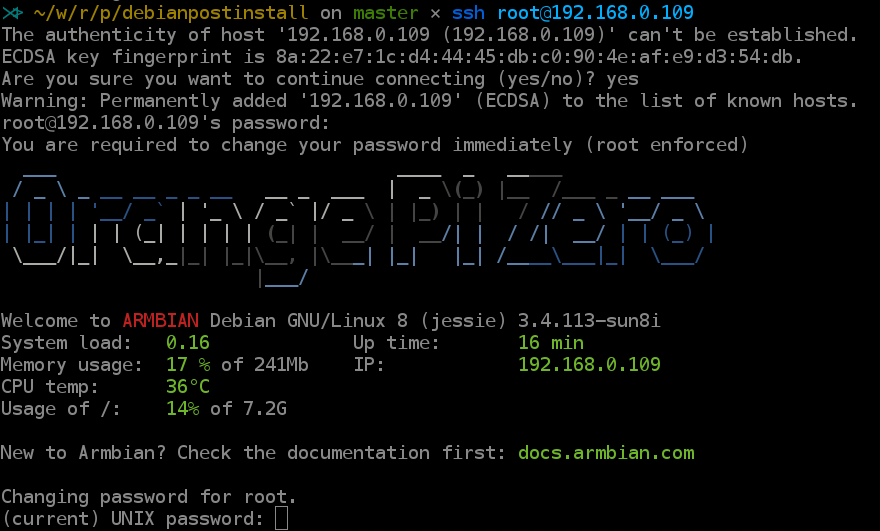
\includegraphics{src/img/OrangePiZero_FirstLogin.png}
\caption{Primer login en \emph{Orange Pi}}
\end{figure}

Lo primero es poner al dia el sistema:

\begin{verbatim}
apt-get update
apt-get upgrade
\end{verbatim}

Si quieres puedes reconfigurar el \emph{time zone}:

\begin{verbatim}
dpgk-reconfigura tzdata
\end{verbatim}

\subsection{Conexión WIFI}\label{conexiuxf3n-wifi}

Vamos a comprobar que todo va bien:

\begin{verbatim}
root@orangepizero:~# iwconfig
lo        no wireless extensions.

tunl0     no wireless extensions.

wlan0     IEEE 802.11bgn  ESSID:off/any
          Mode:Managed  Access Point: Not-Associated   Tx-Power=20 dBm
          Retry  long limit:7   RTS thr:off   Fragment thr:off
          Encryption key:off
          Power Management:on

eth0      no wireless extensions.
\end{verbatim}

Todo tiene buena pinta, vamos a ver si detecta WIFIs:

\begin{verbatim}
root@orangepizero:~# iwlist wlan0  scan |grep ESSID
                    ESSID:"wificlientesR"
                    ESSID:"casa_de_verano"
                    ESSID:"MOVISTAR_BEEF"
                    ESSID:"wificlientesR"
                    ESSID:"R-wlan90"
                    ESSID:"MOVISTAR_BAAF"
                    ESSID:"ababab"
                    ESSID:"WLAN 77"
                    ESSID:"castillo"
                    ESSID:"unaWifi"
                    ESSID:""
                    ESSID:"mikasa"
\end{verbatim}

Para configurar el wifi echamos un ojo al fichero
\texttt{/etc/network/interfaces} pero en ese mismo fichero encontramos
el aviso:

\begin{verbatim}
# Armbian ships with network-manager installed by default. To save you time
# and hassles consider using 'sudo nmtui' instead of configuring Wi-Fi settings
# manually.
\end{verbatim}

Así que basta con ejecutar \texttt{sudo\ nwtui} y ya podemos dar de alta
nuestra wifi (yo la prefiero con IP estática).

\begin{figure}[htbp]
\centering
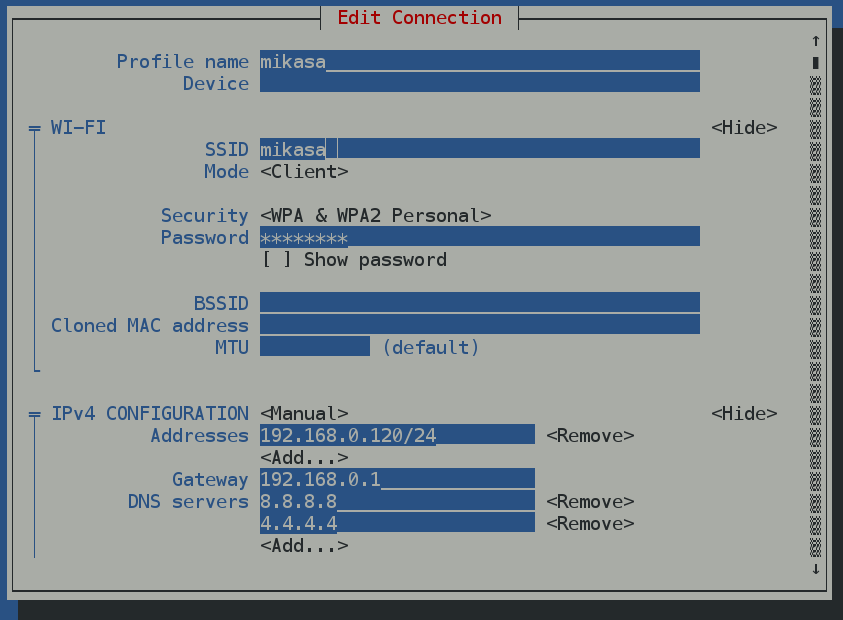
\includegraphics{src/img/OrangePiZero_tmtui.png}
\caption{Configuración WIFI}
\end{figure}

Ejecutamos \texttt{ifconfig} y ya vemos nuestro nuevo interface
configurado:

\begin{verbatim}
ifconfig

wlan0     Link encap:Ethernet  HWaddr a4:7c:f2:9a:97:7c
          inet addr:192.168.0.120  Bcast:192.168.0.255  Mask:255.255.255.0
          inet6 addr: fe80::a67c:f2ff:fe9a:977c/64 Scope:Link
          UP BROADCAST RUNNING MULTICAST  MTU:1500  Metric:1
          RX packets:2 errors:0 dropped:0 overruns:0 frame:0
          TX packets:8 errors:0 dropped:0 overruns:0 carrier:0
          collisions:0 txqueuelen:1000
          RX bytes:328 (328.0 B)  TX bytes:852 (852.0 B)
\end{verbatim}

\section{Referencias}\label{referencias}

\begin{itemize}
\tightlist
\item
  \href{http://www.orangepi.org/}{Página oficial}
\item
  \href{http://www.orangepi.org/downloadresources/}{Recursos oficiales}
  aquí hay imágenes y los esquemáticos
\item
  \href{https://www.aliexpress.com/store/1553371?spm=2114.8147860.0.0.F1q43C}{Tienda
  en Aliexpress}
\item
  \url{http://linux-sunxi.org/Bootable_SD_card}
\item
  \url{https://www.armbian.com/orange-pi-zero/}
\item
  \url{https://docs.armbian.com/User-Guide_Getting-Started/}
\item
  \url{https://docs.armbian.com/Hardware_Allwinner/}
\item
  \href{https://linux-sunxi.org/GPIO}{GPIO} Una explicación de como
  acceder al gpio desde terminal
\item
  \href{https://linux-sunxi.org/Orange_Pi_Zero}{Info variada} Aquí
  tenemos el esquema de pines
\item
  \href{https://forum.armbian.com/index.php/topic/1886-gpio-access-from-user-space/}{GPIO
  desde el espacio de usurario}
\item
  \href{https://forum.armbian.com/index.php/topic/1471-solved-difficulty-accessing-gpio-via-the-sunxi-gpio-export-interface/}{sunxi-gpio}
\end{itemize}

\section{META}\label{meta}

Este documento está escrito en
\href{http://pandoc.org/README.html}{Markdown-Pandoc}. Pandoc es un
sistema muy sencillo de documentación que permite generar múltiples
formatos de salida.

Las fuentes del documento están en el directorio \textbf{doc/src} dentro
del árbol de directorios del proyecto.

Los formatos de salida son el fichero \textbf{README.md} en formato
\emph{Markdown-Github} y los documentos que puedes encontrar en el
directorio \textbf{doc/out} incluyendo un fichero en formato \emph{pdf}.

Los documentos en los distintos formatos de salida se generan
automáticamente sin mas que ejecutar:

\begin{verbatim}
$ cd doc
$ make
\end{verbatim}

Otras opciones que soporta el \textbf{makefile} serían:

\begin{description}
\item[reset]
para regenerar todos los documentos de salida.
\item[clean]
para borrar todos los fichero de salida
\item[pdf, latex, mediawiki, epub, odt, docx]
genera el fichero de salida en el formato especificado: pdf, latex, etc.
etc.
\end{description}

Ejemplos:

\begin{verbatim}
$ make reset
$ make odt
\end{verbatim}

\section{Requisitos}\label{requisitos}

Necesitas tener instalaco \textbf{Pandoc}, hay
\href{https://github.com/brico-labs/pandoc_basico}{una pequeña
introducción} en el el github de BricoLabs.

\section{Licencia}\label{licencia}

\begin{verbatim}

Attribution-ShareAlike 4.0 International

=======================================================================

Creative Commons Corporation ("Creative Commons") is not a law firm and
does not provide legal services or legal advice. Distribution of
Creative Commons public licenses does not create a lawyer-client or
other relationship. Creative Commons makes its licenses and related
information available on an "as-is" basis. Creative Commons gives no
warranties regarding its licenses, any material licensed under their
terms and conditions, or any related information. Creative Commons
disclaims all liability for damages resulting from their use to the
fullest extent possible.

Using Creative Commons Public Licenses

Creative Commons public licenses provide a standard set of terms and
conditions that creators and other rights holders may use to share
original works of authorship and other material subject to copyright
and certain other rights specified in the public license below. The
following considerations are for informational purposes only, are not
exhaustive, and do not form part of our licenses.

     Considerations for licensors: Our public licenses are
     intended for use by those authorized to give the public
     permission to use material in ways otherwise restricted by
     copyright and certain other rights. Our licenses are
     irrevocable. Licensors should read and understand the terms
     and conditions of the license they choose before applying it.
     Licensors should also secure all rights necessary before
     applying our licenses so that the public can reuse the
     material as expected. Licensors should clearly mark any
     material not subject to the license. This includes other CC-
     licensed material, or material used under an exception or
     limitation to copyright. More considerations for licensors:
    wiki.creativecommons.org/Considerations_for_licensors

     Considerations for the public: By using one of our public
     licenses, a licensor grants the public permission to use the
     licensed material under specified terms and conditions. If
     the licensor's permission is not necessary for any reason--for
     example, because of any applicable exception or limitation to
     copyright--then that use is not regulated by the license. Our
     licenses grant only permissions under copyright and certain
     other rights that a licensor has authority to grant. Use of
     the licensed material may still be restricted for other
     reasons, including because others have copyright or other
     rights in the material. A licensor may make special requests,
     such as asking that all changes be marked or described.
     Although not required by our licenses, you are encouraged to
     respect those requests where reasonable. More_considerations
     for the public: 
    wiki.creativecommons.org/Considerations_for_licensees

=======================================================================

Creative Commons Attribution-ShareAlike 4.0 International Public
License

By exercising the Licensed Rights (defined below), You accept and agree
to be bound by the terms and conditions of this Creative Commons
Attribution-ShareAlike 4.0 International Public License ("Public
License"). To the extent this Public License may be interpreted as a
contract, You are granted the Licensed Rights in consideration of Your
acceptance of these terms and conditions, and the Licensor grants You
such rights in consideration of benefits the Licensor receives from
making the Licensed Material available under these terms and
conditions.


Section 1 -- Definitions.

  a. Adapted Material means material subject to Copyright and Similar
     Rights that is derived from or based upon the Licensed Material
     and in which the Licensed Material is translated, altered,
     arranged, transformed, or otherwise modified in a manner requiring
     permission under the Copyright and Similar Rights held by the
     Licensor. For purposes of this Public License, where the Licensed
     Material is a musical work, performance, or sound recording,
     Adapted Material is always produced where the Licensed Material is
     synched in timed relation with a moving image.

  b. Adapter's License means the license You apply to Your Copyright
     and Similar Rights in Your contributions to Adapted Material in
     accordance with the terms and conditions of this Public License.

  c. BY-SA Compatible License means a license listed at
     creativecommons.org/compatiblelicenses, approved by Creative
     Commons as essentially the equivalent of this Public License.

  d. Copyright and Similar Rights means copyright and/or similar rights
     closely related to copyright including, without limitation,
     performance, broadcast, sound recording, and Sui Generis Database
     Rights, without regard to how the rights are labeled or
     categorized. For purposes of this Public License, the rights
     specified in Section 2(b)(1)-(2) are not Copyright and Similar
     Rights.

  e. Effective Technological Measures means those measures that, in the
     absence of proper authority, may not be circumvented under laws
     fulfilling obligations under Article 11 of the WIPO Copyright
     Treaty adopted on December 20, 1996, and/or similar international
     agreements.

  f. Exceptions and Limitations means fair use, fair dealing, and/or
     any other exception or limitation to Copyright and Similar Rights
     that applies to Your use of the Licensed Material.

  g. License Elements means the license attributes listed in the name
     of a Creative Commons Public License. The License Elements of this
     Public License are Attribution and ShareAlike.

  h. Licensed Material means the artistic or literary work, database,
     or other material to which the Licensor applied this Public
     License.

  i. Licensed Rights means the rights granted to You subject to the
     terms and conditions of this Public License, which are limited to
     all Copyright and Similar Rights that apply to Your use of the
     Licensed Material and that the Licensor has authority to license.

  j. Licensor means the individual(s) or entity(ies) granting rights
     under this Public License.

  k. Share means to provide material to the public by any means or
     process that requires permission under the Licensed Rights, such
     as reproduction, public display, public performance, distribution,
     dissemination, communication, or importation, and to make material
     available to the public including in ways that members of the
     public may access the material from a place and at a time
     individually chosen by them.

  l. Sui Generis Database Rights means rights other than copyright
     resulting from Directive 96/9/EC of the European Parliament and of
     the Council of 11 March 1996 on the legal protection of databases,
     as amended and/or succeeded, as well as other essentially
     equivalent rights anywhere in the world.

  m. You means the individual or entity exercising the Licensed Rights
     under this Public License. Your has a corresponding meaning.


Section 2 -- Scope.

  a. License grant.

       1. Subject to the terms and conditions of this Public License,
          the Licensor hereby grants You a worldwide, royalty-free,
          non-sublicensable, non-exclusive, irrevocable license to
          exercise the Licensed Rights in the Licensed Material to:

            a. reproduce and Share the Licensed Material, in whole or
               in part; and

            b. produce, reproduce, and Share Adapted Material.

       2. Exceptions and Limitations. For the avoidance of doubt, where
          Exceptions and Limitations apply to Your use, this Public
          License does not apply, and You do not need to comply with
          its terms and conditions.

       3. Term. The term of this Public License is specified in Section
          6(a).

       4. Media and formats; technical modifications allowed. The
          Licensor authorizes You to exercise the Licensed Rights in
          all media and formats whether now known or hereafter created,
          and to make technical modifications necessary to do so. The
          Licensor waives and/or agrees not to assert any right or
          authority to forbid You from making technical modifications
          necessary to exercise the Licensed Rights, including
          technical modifications necessary to circumvent Effective
          Technological Measures. For purposes of this Public License,
          simply making modifications authorized by this Section 2(a)
          (4) never produces Adapted Material.

       5. Downstream recipients.

            a. Offer from the Licensor -- Licensed Material. Every
               recipient of the Licensed Material automatically
               receives an offer from the Licensor to exercise the
               Licensed Rights under the terms and conditions of this
               Public License.

            b. Additional offer from the Licensor -- Adapted Material.
               Every recipient of Adapted Material from You
               automatically receives an offer from the Licensor to
               exercise the Licensed Rights in the Adapted Material
               under the conditions of the Adapter's License You apply.

            c. No downstream restrictions. You may not offer or impose
               any additional or different terms or conditions on, or
               apply any Effective Technological Measures to, the
               Licensed Material if doing so restricts exercise of the
               Licensed Rights by any recipient of the Licensed
               Material.

       6. No endorsement. Nothing in this Public License constitutes or
          may be construed as permission to assert or imply that You
          are, or that Your use of the Licensed Material is, connected
          with, or sponsored, endorsed, or granted official status by,
          the Licensor or others designated to receive attribution as
          provided in Section 3(a)(1)(A)(i).

  b. Other rights.

       1. Moral rights, such as the right of integrity, are not
          licensed under this Public License, nor are publicity,
          privacy, and/or other similar personality rights; however, to
          the extent possible, the Licensor waives and/or agrees not to
          assert any such rights held by the Licensor to the limited
          extent necessary to allow You to exercise the Licensed
          Rights, but not otherwise.

       2. Patent and trademark rights are not licensed under this
          Public License.

       3. To the extent possible, the Licensor waives any right to
          collect royalties from You for the exercise of the Licensed
          Rights, whether directly or through a collecting society
          under any voluntary or waivable statutory or compulsory
          licensing scheme. In all other cases the Licensor expressly
          reserves any right to collect such royalties.


Section 3 -- License Conditions.

Your exercise of the Licensed Rights is expressly made subject to the
following conditions.

  a. Attribution.

       1. If You Share the Licensed Material (including in modified
          form), You must:

            a. retain the following if it is supplied by the Licensor
               with the Licensed Material:

                 i. identification of the creator(s) of the Licensed
                    Material and any others designated to receive
                    attribution, in any reasonable manner requested by
                    the Licensor (including by pseudonym if
                    designated);

                ii. a copyright notice;

               iii. a notice that refers to this Public License;

                iv. a notice that refers to the disclaimer of
                    warranties;

                 v. a URI or hyperlink to the Licensed Material to the
                    extent reasonably practicable;

            b. indicate if You modified the Licensed Material and
               retain an indication of any previous modifications; and

            c. indicate the Licensed Material is licensed under this
               Public License, and include the text of, or the URI or
               hyperlink to, this Public License.

       2. You may satisfy the conditions in Section 3(a)(1) in any
          reasonable manner based on the medium, means, and context in
          which You Share the Licensed Material. For example, it may be
          reasonable to satisfy the conditions by providing a URI or
          hyperlink to a resource that includes the required
          information.

       3. If requested by the Licensor, You must remove any of the
          information required by Section 3(a)(1)(A) to the extent
          reasonably practicable.

  b. ShareAlike.

     In addition to the conditions in Section 3(a), if You Share
     Adapted Material You produce, the following conditions also apply.

       1. The Adapter's License You apply must be a Creative Commons
          license with the same License Elements, this version or
          later, or a BY-SA Compatible License.

       2. You must include the text of, or the URI or hyperlink to, the
          Adapter's License You apply. You may satisfy this condition
          in any reasonable manner based on the medium, means, and
          context in which You Share Adapted Material.

       3. You may not offer or impose any additional or different terms
          or conditions on, or apply any Effective Technological
          Measures to, Adapted Material that restrict exercise of the
          rights granted under the Adapter's License You apply.


Section 4 -- Sui Generis Database Rights.

Where the Licensed Rights include Sui Generis Database Rights that
apply to Your use of the Licensed Material:

  a. for the avoidance of doubt, Section 2(a)(1) grants You the right
     to extract, reuse, reproduce, and Share all or a substantial
     portion of the contents of the database;

  b. if You include all or a substantial portion of the database
     contents in a database in which You have Sui Generis Database
     Rights, then the database in which You have Sui Generis Database
     Rights (but not its individual contents) is Adapted Material,

     including for purposes of Section 3(b); and
  c. You must comply with the conditions in Section 3(a) if You Share
     all or a substantial portion of the contents of the database.

For the avoidance of doubt, this Section 4 supplements and does not
replace Your obligations under this Public License where the Licensed
Rights include other Copyright and Similar Rights.


Section 5 -- Disclaimer of Warranties and Limitation of Liability.

  a. UNLESS OTHERWISE SEPARATELY UNDERTAKEN BY THE LICENSOR, TO THE
     EXTENT POSSIBLE, THE LICENSOR OFFERS THE LICENSED MATERIAL AS-IS
     AND AS-AVAILABLE, AND MAKES NO REPRESENTATIONS OR WARRANTIES OF
     ANY KIND CONCERNING THE LICENSED MATERIAL, WHETHER EXPRESS,
     IMPLIED, STATUTORY, OR OTHER. THIS INCLUDES, WITHOUT LIMITATION,
     WARRANTIES OF TITLE, MERCHANTABILITY, FITNESS FOR A PARTICULAR
     PURPOSE, NON-INFRINGEMENT, ABSENCE OF LATENT OR OTHER DEFECTS,
     ACCURACY, OR THE PRESENCE OR ABSENCE OF ERRORS, WHETHER OR NOT
     KNOWN OR DISCOVERABLE. WHERE DISCLAIMERS OF WARRANTIES ARE NOT
     ALLOWED IN FULL OR IN PART, THIS DISCLAIMER MAY NOT APPLY TO YOU.

  b. TO THE EXTENT POSSIBLE, IN NO EVENT WILL THE LICENSOR BE LIABLE
     TO YOU ON ANY LEGAL THEORY (INCLUDING, WITHOUT LIMITATION,
     NEGLIGENCE) OR OTHERWISE FOR ANY DIRECT, SPECIAL, INDIRECT,
     INCIDENTAL, CONSEQUENTIAL, PUNITIVE, EXEMPLARY, OR OTHER LOSSES,
     COSTS, EXPENSES, OR DAMAGES ARISING OUT OF THIS PUBLIC LICENSE OR
     USE OF THE LICENSED MATERIAL, EVEN IF THE LICENSOR HAS BEEN
     ADVISED OF THE POSSIBILITY OF SUCH LOSSES, COSTS, EXPENSES, OR
     DAMAGES. WHERE A LIMITATION OF LIABILITY IS NOT ALLOWED IN FULL OR
     IN PART, THIS LIMITATION MAY NOT APPLY TO YOU.

  c. The disclaimer of warranties and limitation of liability provided
     above shall be interpreted in a manner that, to the extent
     possible, most closely approximates an absolute disclaimer and
     waiver of all liability.


Section 6 -- Term and Termination.

  a. This Public License applies for the term of the Copyright and
     Similar Rights licensed here. However, if You fail to comply with
     this Public License, then Your rights under this Public License
     terminate automatically.

  b. Where Your right to use the Licensed Material has terminated under
     Section 6(a), it reinstates:

       1. automatically as of the date the violation is cured, provided
          it is cured within 30 days of Your discovery of the
          violation; or

       2. upon express reinstatement by the Licensor.

     For the avoidance of doubt, this Section 6(b) does not affect any
     right the Licensor may have to seek remedies for Your violations
     of this Public License.

  c. For the avoidance of doubt, the Licensor may also offer the
     Licensed Material under separate terms or conditions or stop
     distributing the Licensed Material at any time; however, doing so
     will not terminate this Public License.

  d. Sections 1, 5, 6, 7, and 8 survive termination of this Public
     License.


Section 7 -- Other Terms and Conditions.

  a. The Licensor shall not be bound by any additional or different
     terms or conditions communicated by You unless expressly agreed.

  b. Any arrangements, understandings, or agreements regarding the
     Licensed Material not stated herein are separate from and
     independent of the terms and conditions of this Public License.


Section 8 -- Interpretation.

  a. For the avoidance of doubt, this Public License does not, and
     shall not be interpreted to, reduce, limit, restrict, or impose
     conditions on any use of the Licensed Material that could lawfully
     be made without permission under this Public License.

  b. To the extent possible, if any provision of this Public License is
     deemed unenforceable, it shall be automatically reformed to the
     minimum extent necessary to make it enforceable. If the provision
     cannot be reformed, it shall be severed from this Public License
     without affecting the enforceability of the remaining terms and
     conditions.

  c. No term or condition of this Public License will be waived and no
     failure to comply consented to unless expressly agreed to by the
     Licensor.

  d. Nothing in this Public License constitutes or may be interpreted
     as a limitation upon, or waiver of, any privileges and immunities
     that apply to the Licensor or You, including from the legal
     processes of any jurisdiction or authority.


=======================================================================

Creative Commons is not a party to its public
licenses. Notwithstanding, Creative Commons may elect to apply one of
its public licenses to material it publishes and in those instances
will be considered the “Licensor.” The text of the Creative Commons
public licenses is dedicated to the public domain under the CC0 Public
Domain Dedication. Except for the limited purpose of indicating that
material is shared under a Creative Commons public license or as
otherwise permitted by the Creative Commons policies published at
creativecommons.org/policies, Creative Commons does not authorize the
use of the trademark "Creative Commons" or any other trademark or logo
of Creative Commons without its prior written consent including,
without limitation, in connection with any unauthorized modifications
to any of its public licenses or any other arrangements,
understandings, or agreements concerning use of licensed material. For
the avoidance of doubt, this paragraph does not form part of the
public licenses.

Creative Commons may be contacted at creativecommons.org.
\end{verbatim}

\end{document}
